\documentclass[12pt]{article}

\usepackage{geometry}
\geometry{a4paper, left=1in, right=1in, top=1in, bottom=1in}
\usepackage{amsmath}
\usepackage{amsmath,amsfonts,amssymb}
\usepackage{graphicx}
\usepackage{subcaption}
\usepackage{enumitem}
\usepackage{titlesec}
\usepackage{fancyhdr}
\usepackage{hyperref}
\usepackage{floatrow}
\usepackage{geometry}
\usepackage{fancyhdr}
\usepackage{empheq}
\usepackage[svgnames]{xcolor}
\usepackage{xpatch}

\makeatletter
\newcommand{\colorboxed}[1]{\fcolorbox{Black}{White}{\m@th$\displaystyle#1$}}
\xpatchcmd{\@Aboxed}{\boxed}{\colorboxed}{}{}
\makeatother

\title{{\bf CS663 Assignment 3}}
\author{Saksham Rathi, Kavya Gupta, Shravan Srinivasa Raghavan}
\date{September 2024}
\begin{document}
\maketitle
\clearpage
\section*{Question 3}
\addcontentsline{toc}{section}{Question 3}
Here are the original and the noisy versions of the images:
\begin{figure}[h]
    \centering
    % First subfigure
    \begin{subfigure}[b]{0.3\textwidth}
        \centering
        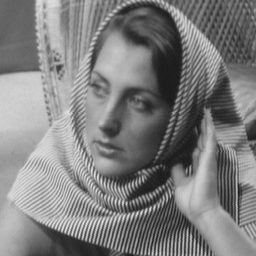
\includegraphics[width=\textwidth]{../images/barbara256.png}
        \caption{Original}
        \label{fig:subfig1}
    \end{subfigure}
    % Second subfigure
    \begin{subfigure}[b]{0.3\textwidth}
        \centering
        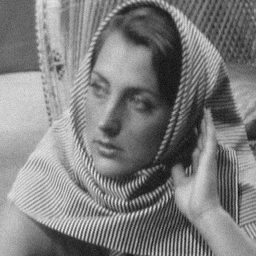
\includegraphics[width=\textwidth]{../images/noisy_barbara256.png}
        \caption{Noisy (sigma=5)}
        \label{fig:subfig2}
    \end{subfigure}
    \caption{Versions of barbara image}
    \label{fig:overall}
\end{figure}

\begin{figure}[h]
    \centering
    % First subfigure
    \begin{subfigure}[b]{0.3\textwidth}
        \centering
        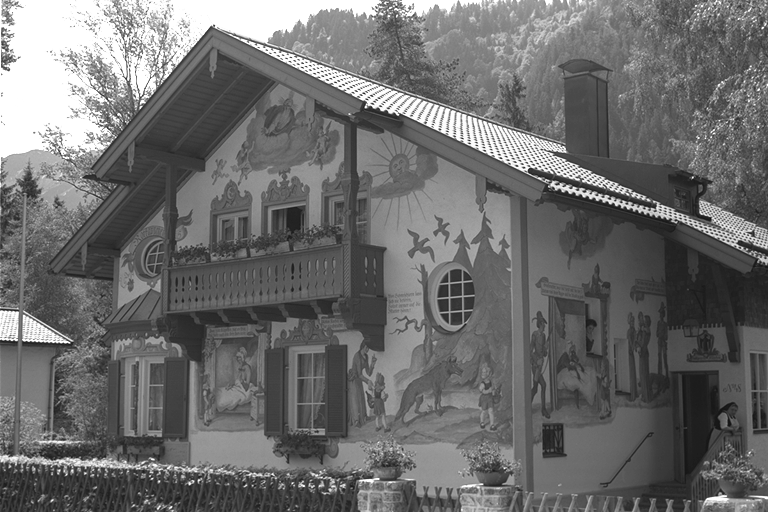
\includegraphics[width=\textwidth]{../images/kodak24.png}
        \caption{Original}
        \label{fig:subfig1}
    \end{subfigure}
    % Second subfigure
    \begin{subfigure}[b]{0.3\textwidth}
        \centering
        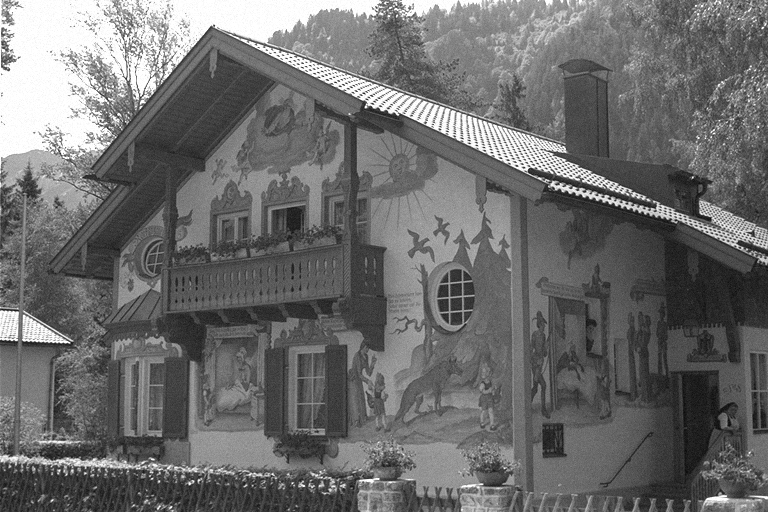
\includegraphics[width=\textwidth]{../images/noisy_kodak24.png}
        \caption{Noisy (sigma=5)}
        \label{fig:subfig2}
    \end{subfigure}
    \caption{Versions of kodak image}
    \label{fig:kodak}
\end{figure}

The code for this question is present in {../code/myMainScript.m}, \\ {../code/mybilateralfilter.m} and {../code/mymeanshiftfilter.m}. The window size of the bilateral filter and the meanshift filter is chosen to be $2\times [3*\sigma_s] + 1$, where $[]$ denotes the ceiling function.


Here are the results of applying bilateral filter on noisy ($\sigma = 5$) barbara image with various values of $\sigma_s$ and $\sigma_r$:

\begin{figure}[h]
    \centering
    % First subfigure
    \begin{subfigure}[b]{0.24\textwidth}
        \centering
        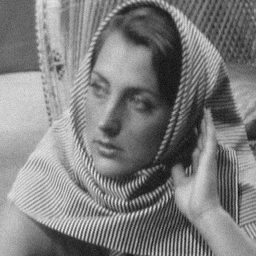
\includegraphics[width=\textwidth]{../images/noisy_barbara256.png}
        \caption{sigma=5}
        \label{Noisy (sigma=5)}
    \end{subfigure}
    % Second subfigure
    \begin{subfigure}[b]{0.24\textwidth}
        \centering
        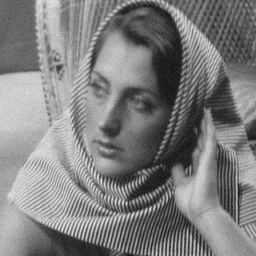
\includegraphics[width=\textwidth]{../images/filtered_barbara256_bilateral_sigma_s_2_sigma_r_2.png}
        \caption{$\sigma_s=2;\sigma_r=2$}
        \label{fig:subfig2}
    \end{subfigure}
    % Third subfigure
    \begin{subfigure}[b]{0.24\textwidth}
        \centering
        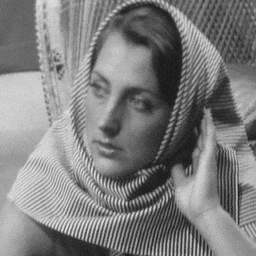
\includegraphics[width=\textwidth]{../images/filtered_barbara256_bilateral_sigma_s_3_sigma_r_15.png}
        \caption{$\sigma_s=3;\sigma_r=15$}
        \label{fig:subfig3}
    \end{subfigure}
    \begin{subfigure}[b]{0.24\textwidth}
        \centering
        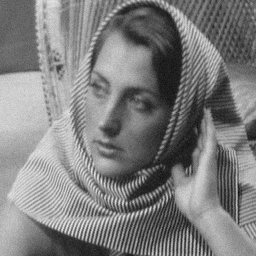
\includegraphics[width=\textwidth]{../images/filtered_barbara256_bilateral_sigma_s_15_sigma_r_3.png}
        \caption{$\sigma_s=15;\sigma_r=3$}
        \label{fig:subfig3}
    \end{subfigure}
    
    \caption{Bilateral Versions of barbara image (sigma=5)}
    \label{fig:overall}
\end{figure}


Here are the results of applying mean-shift filter on noisy ($\sigma = 5$) barbara image with various values of $\sigma_s$ and $\sigma_r$:

\begin{figure}[h]
    \centering
    % First subfigure
    \begin{subfigure}[b]{0.24\textwidth}
        \centering
        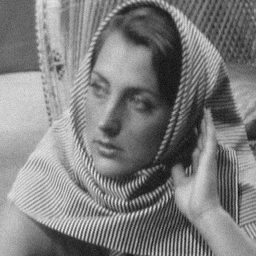
\includegraphics[width=\textwidth]{../images/noisy_barbara256.png}
        \caption{sigma=5}
        \label{Noisy (sigma=5)}
    \end{subfigure}
    % Second subfigure
    \begin{subfigure}[b]{0.24\textwidth}
        \centering
        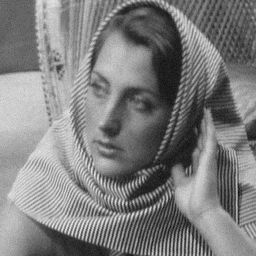
\includegraphics[width=\textwidth]{../images/filtered_barbara256_meanshift_sigma_s_2_sigma_r_2.png}
        \caption{$\sigma_s=2;\sigma_r=2$}
        \label{fig:subfig2}
    \end{subfigure}
    % Third subfigure
    \begin{subfigure}[b]{0.24\textwidth}
        \centering
        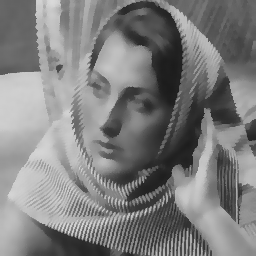
\includegraphics[width=\textwidth]{../images/filtered_barbara256_meanshift_sigma_s_3_sigma_r_15.png}
        \caption{$\sigma_s=3;\sigma_r=15$}
        \label{fig:subfig3}
    \end{subfigure}
    \begin{subfigure}[b]{0.24\textwidth}
        \centering
        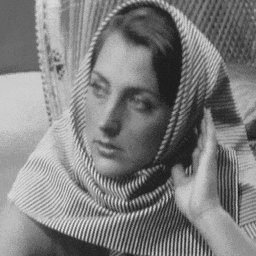
\includegraphics[width=\textwidth]{../images/filtered_barbara256_meanshift_sigma_s_15_sigma_r_3.png}
        \caption{$\sigma_s=15;\sigma_r=3$}
        \label{fig:subfig3}
    \end{subfigure}
    
    \caption{Mean-shift Versions of kodak image (sigma=5)}
    \label{fig:overall}
\end{figure}


Here are the results of applying bilateral filter on noisy ($\sigma = 5$) kodak image with various values of $\sigma_s$ and $\sigma_r$:

\begin{figure}[h]
    \centering
    % First subfigure
    \begin{subfigure}[b]{0.24\textwidth}
        \centering
        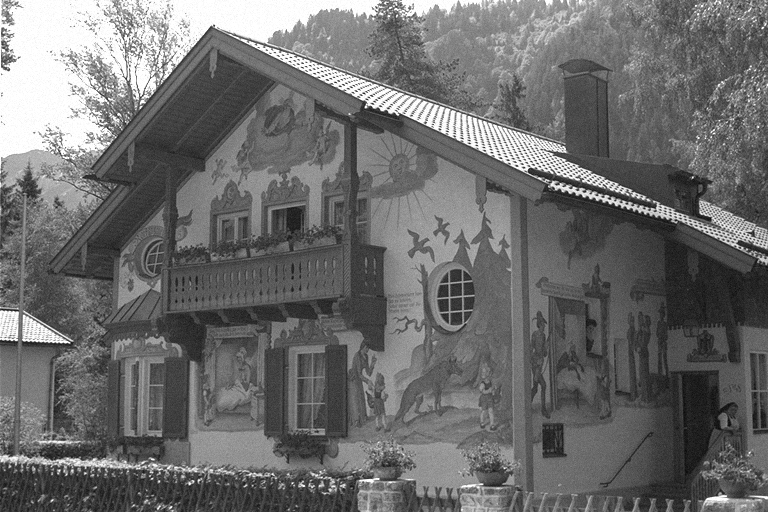
\includegraphics[width=\textwidth]{../images/noisy_kodak24.png}
        \caption{sigma=5}
        \label{Noisy (sigma=5)}
    \end{subfigure}
    % Second subfigure
    \begin{subfigure}[b]{0.24\textwidth}
        \centering
        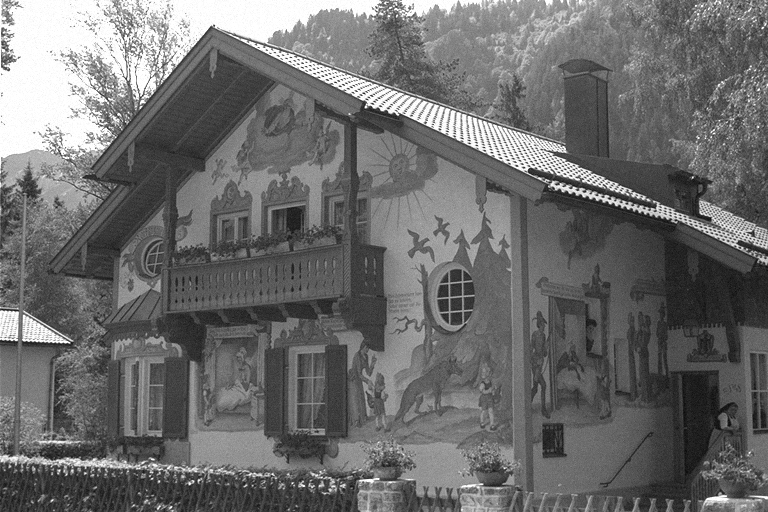
\includegraphics[width=\textwidth]{../images/filtered_kodak24_bilateral_sigma_s_2_sigma_r_2.png}
        \caption{$\sigma_s=2;\sigma_r=2$}
        \label{fig:subfig2}
    \end{subfigure}
    % Third subfigure
    \begin{subfigure}[b]{0.24\textwidth}
        \centering
        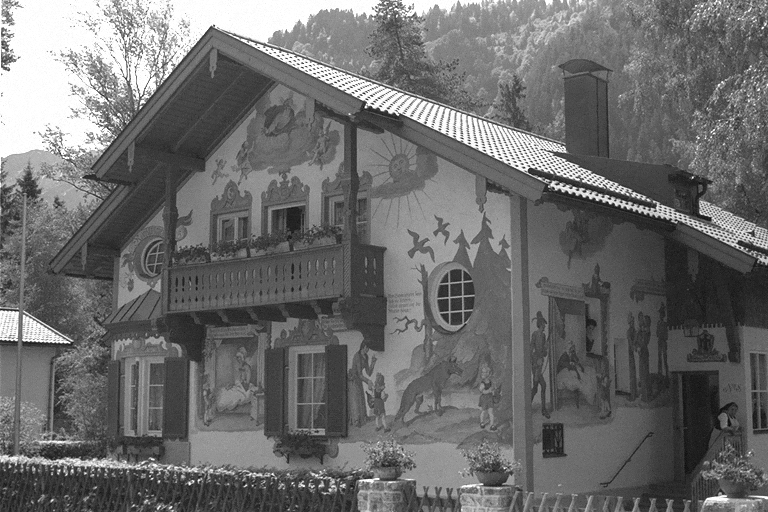
\includegraphics[width=\textwidth]{../images/filtered_kodak24_bilateral_sigma_s_3_sigma_r_15.png}
        \caption{$\sigma_s=3;\sigma_r=15$}
        \label{fig:subfig3}
    \end{subfigure}
    \begin{subfigure}[b]{0.24\textwidth}
        \centering
        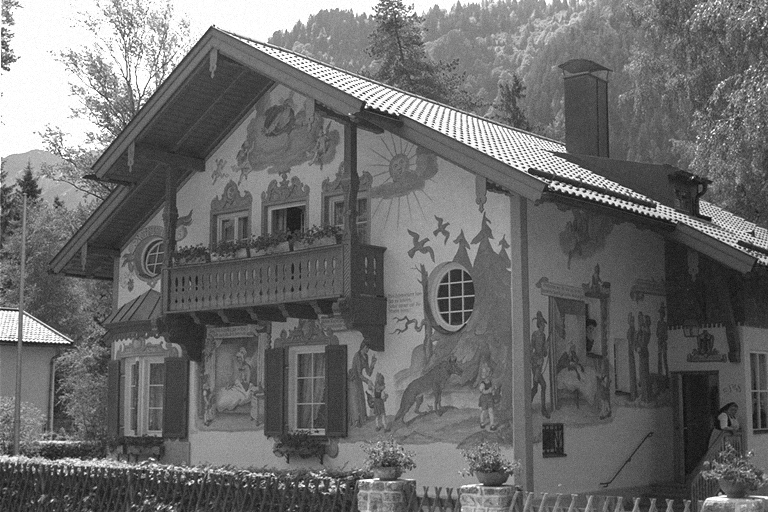
\includegraphics[width=\textwidth]{../images/filtered_kodak24_bilateral_sigma_s_15_sigma_r_3.png}
        \caption{$\sigma_s=15;\sigma_r=3$}
        \label{fig:subfig3}
    \end{subfigure}
    
    \caption{Bilateral Versions of kodak image (sigma=5)}
    \label{fig:overall}
\end{figure}


Here are the results of applying mean-shift filter on noisy ($\sigma = 5$) kodak image with various values of $\sigma_s$ and $\sigma_r$:

\begin{figure}[h]
    \centering
    % First subfigure
    \begin{subfigure}[b]{0.24\textwidth}
        \centering
        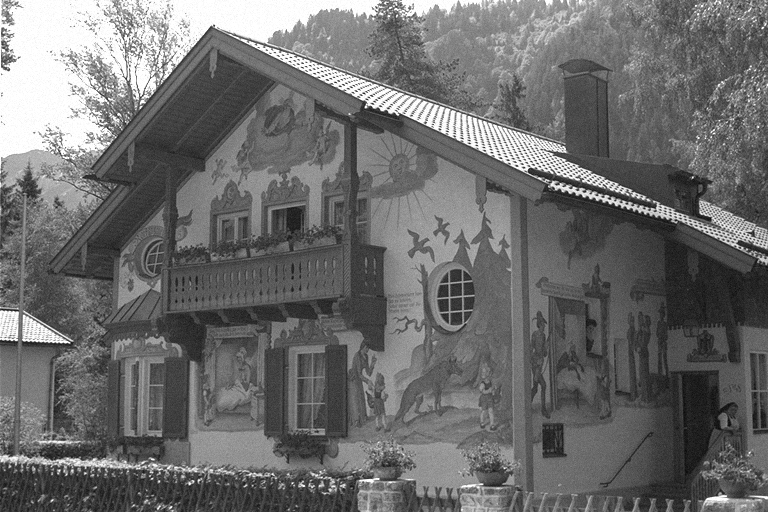
\includegraphics[width=\textwidth]{../images/noisy_kodak24.png}
        \caption{sigma=5}
        \label{Noisy (sigma=5)}
    \end{subfigure}
    % Second subfigure
    \begin{subfigure}[b]{0.24\textwidth}
        \centering
        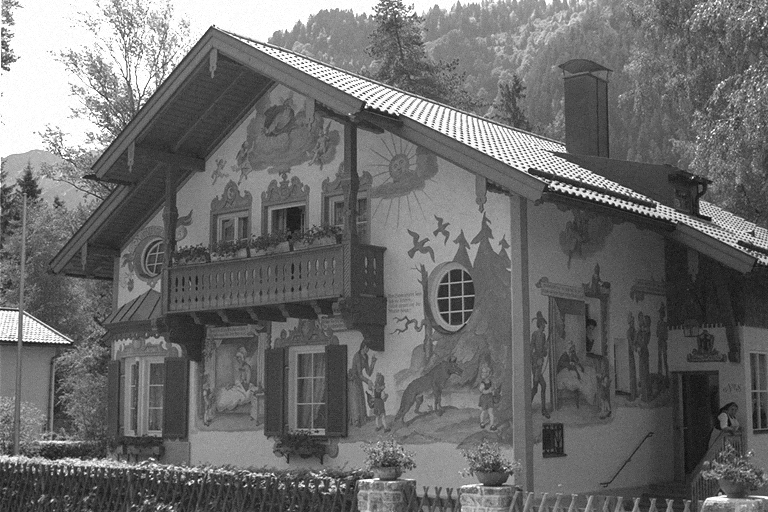
\includegraphics[width=\textwidth]{../images/filtered_kodak24_meanshift_sigma_s_2_sigma_r_2.png}
        \caption{$\sigma_s=2;\sigma_r=2$}
        \label{fig:subfig2}
    \end{subfigure}
    % Third subfigure
    \begin{subfigure}[b]{0.24\textwidth}
        \centering
        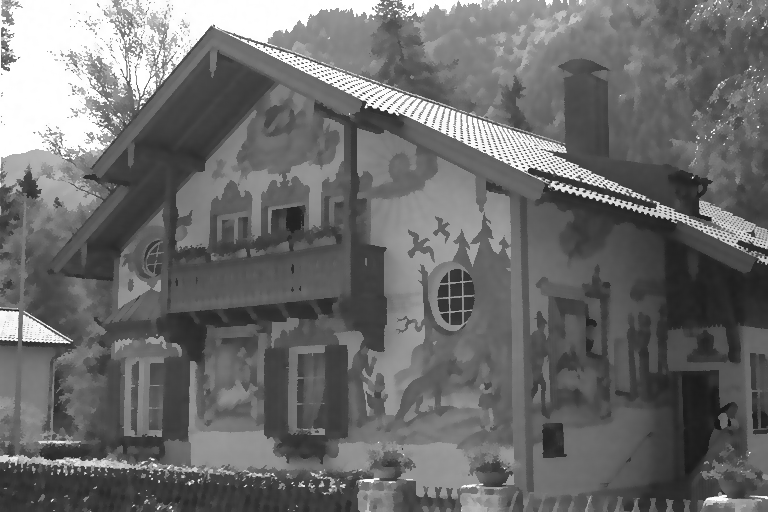
\includegraphics[width=\textwidth]{../images/filtered_kodak24_meanshift_sigma_s_3_sigma_r_15.png}
        \caption{$\sigma_s=3;\sigma_r=15$}
        \label{fig:subfig3}
    \end{subfigure}
    \begin{subfigure}[b]{0.24\textwidth}
        \centering
        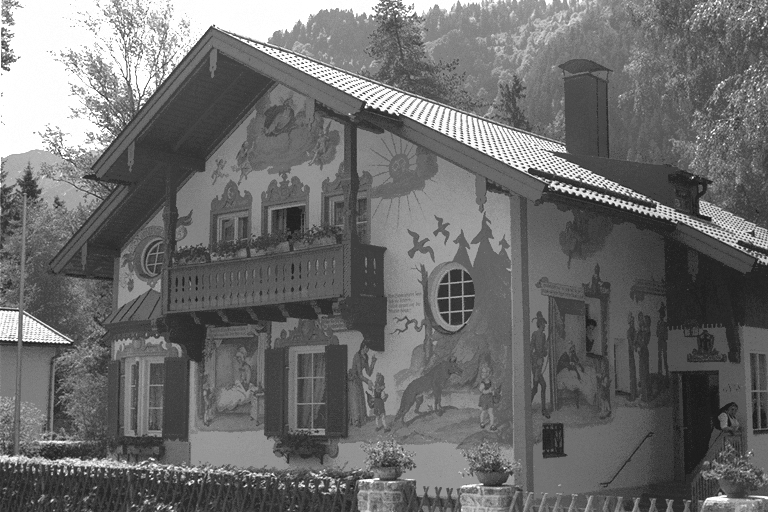
\includegraphics[width=\textwidth]{../images/filtered_kodak24_meanshift_sigma_s_15_sigma_r_3.png}
        \caption{$\sigma_s=15;\sigma_r=3$}
        \label{fig:subfig3}
    \end{subfigure}
    
    \caption{Mean-shift Versions of kodak image (sigma=5)}
    \label{fig:overall}
\end{figure}

\end{document}